\chapter{Gestione della memoria}

In questo capitolo si parlerà della gestione della memoria nei sistemi operativi, in particolare si analizzeranno gli spazi di indirizzamento, l'allocazione contigua, la paginazione, la segmentazione e la segmentazione con paginazione. Si analizzeranno anche le problematiche legate alla gestione della memoria, e le tecniche di allocazione della memoria. Si parlerà anche della memoria virtuale e delle tecniche di swapping, e si analizzeranno i problemi legati alla frammentazione della memoria. Infine si parlerà della gestione della memoria nei sistemi operativi moderni, e delle tecniche di allocazione della memoria nei sistemi operativi a \textit{micro-kernel}.

\section{Introduzione}
    Per rendere un sistema operativo efficiente la condivisione della memoria deve essere gestita in modo da evitare conflitti tra i processi ed efficienti.
    \paragraph{Problematiche}
        Le problematiche che un buon sistema operativo deve affrontare in merito alla gestione della memoria sono:
        \begin{itemize}
            \item Allocazione della memoria ai singoli \textit{job}
            \item Protezione dello spazio di indirizzamento
            \item Condivisione dello spazio di indirizzamento
            \item Nei sistemi operativi moderni: Gestione della memoria virtuale (\textit{swap})
        \end{itemize}
        Tutti questi problemi devono obbligatoriamente essere affrontati in modo, oltre che efficiente, anche sicuro per evitare che un processo possa accedere alla memoria di un altro processo o di un dispositivo e compromettere la stabilità del sistema e/o la sicurezza dei dati.
    \subsection{Dal programma al processo}
        Ogni programma prima di essere eseguito deve essere caricato in memoria e trasformato in un processo. Il sistema operativo deve successivamente prelevare le istruzioni in memoria sulla base del \texttt{PC} (\textit{Program Counter}) e caricare i dati necessari per l'esecuzione del programma. Quando questo è terminato, il sistema operativo deve liberare la memoria occupata dal processo e restituirla al sistema. La creazione di un processo è quindi un'operazione complessa che richiede l'allocazione di risorse e la gestione della memoria.\newline
        Prima di trasformare un programma in un processo, ci sono diverse operazioni da eseguire, in ognuna di queste operazioni possono esserci diverse semantiche degli indirizzi (spazio logico / spazio fisico), solitamente quando si scrive il codice sorgente si fa riferimento a indirizzi logici, mentre quando il codice viene eseguito si deve fare riferimento a indirizzi fisici.\newline
        Il compilatore traduce gli indirizzi logici in indirizzi simbolici ri-locabili, il linker o il loader si occupano di tradurre gli indirizzi ri-locabili in indirizzi assoluti, infine il sistema operativo si occupa di tradurre gli indirizzi assoluti in indirizzi fisici.\newline
        L'insieme delle operazioni che vengono eseguite per trasformare gli indirizzi simbolici in indirizzi assoluti è detto \textbf{\textit{binding}}.
        \subsubsection{\textit{Binding} \& Indirizzi}
            Il \textit{binding} può avvenire in diversi momenti, e a seconda di quando avviene il \textit{binding} si può dividere in \textit{binding} statico e \textit{binding} dinamico:
            \begin{itemize}
                \item \textbf{\textit{Binding} a \textit{compile time}}: il \textit{binding} avviene durante la compilazione del programma, gli indirizzi simbolici vengono tradotti in indirizzi assoluti e il programma viene caricato in memoria con gli indirizzi assoluti. Questo tipo di \textit{binding} è molto veloce, ma non permette di modificare il programma una volta compilato. Questo tipo di \textit{binding} è della categoria del \textit{binding} statico.
                \item \textbf{\textit{Binding} a \textit{load time}}: il \textit{binding} avviene durante il caricamento del programma in memoria, gli indirizzi simbolici vengono tradotti in indirizzi assoluti e il programma viene caricato in memoria con gli indirizzi assoluti. Questo tipo di \text{binding} richiede che gli indirizzi siano ri-locabili, e in questo caso vengono usati indirizzi relativi alla posizione di memoria in cui il programma viene caricato. Questo tipo di \textit{binding} è della categoria del \textit{binding} statico in quanto se il programma viene caricato in una posizione di memoria diversa da quella prevista, il sistema operativo deve modificare gli indirizzi assoluti in indirizzi relativi alla nuova posizione di memoria.
                \item \textbf{\textit{Binding} a \textit{run time}}: il \textit{binding} avviene durante l'esecuzione del programma, gli indirizzi simbolici vengono tradotti in indirizzi assoluti ed il programma può essere caricato in memoria in qualsiasi posizione e spostato in memoria durante l'esecuzione. Questo tipo di \textit{binding} è della categoria del \textit{binding} dinamico ma richiede del supporto \textit{hardware} aggiuntivo.
            \end{itemize}
        \subsubsection{Collegamento (\textit{linking})}
            Un altro passaggio prerequisito alla creazione di un processo è il \textit{linking}, ovvero l'associazione di un programma a tutte le librerie e i moduli necessari. Questo passaggio può avvenire in due modi:
            \begin{itemize}
                \item \textbf{\textit{Linking} statico}: il \textit{linking} avviene durante la compilazione del programma, le librerie e i moduli necessari vengono inclusi per intero nel programma e il programma viene caricato in memoria con tutte le librerie e i moduli necessari. Questo tipo di \textit{linking} è molto veloce, ma aumenta la dimensione del programma e richiede più memoria. Inoltre se una libreria o un modulo viene aggiornato, il programma deve essere ricompilato per utilizzare la nuova versione della libreria o del modulo, oltre al fatto che se non si usano tutte le funzioni di una libreria, il programma occupa più memoria del necessario.
                \item \textbf{\textit{Linking} dinamico}: il \textit{linking} avviene durante l'esecuzione del programma, le librerie e i moduli necessari vengono caricati in memoria solo quando sono necessari e il programma viene caricato in memoria con i riferimenti alle librerie e ai moduli necessari. Questo tipo di \textit{linking} è più lento, ma riduce la dimensione del programma e richiede meno memoria. Inoltre se una libreria o un modulo viene aggiornato, il programma non deve essere ricompilato per utilizzare la nuova versione della libreria o del modulo.
            \end{itemize}
            Il \textit{linking} statico è più veloce, ma richiede più memoria e non permette di aggiornare le librerie e i moduli senza ricompilare il programma. Il \textit{linking} dinamico è più lento, ma richiede meno memoria e permette di aggiornare le librerie e i moduli senza ricompilare il programma.
        \subsubsection{Caricamento (\textit{loading})}
            Il caricamento è l'operazione che permette di caricare un programma in memoria e prepararlo per l'esecuzione. Il caricamento può avvenire in due modi:
            \begin{itemize}
                \item \textbf{\textit{Loading} statico}: l'intero programma viene caricato in memoria in un'unica operazione, il programma viene caricato in memoria con gli indirizzi assoluti e il programma viene eseguito. Questo tipo di \textit{loading} è molto veloce, ma richiede che il programma sia di dimensioni fisse e non permette di modificare il programma una volta caricato in memoria.
                \item \textbf{\textit{Loading} dinamico}: il caricamento di alcuni moduli avviene in modo dinamico, ovvero il programma viene caricato in memoria in più operazioni quando sono necessari. Questo tipo di \textit{loading} è più lento, ma permette di caricare solo i moduli necessari e di modificare il programma una volta caricato in memoria. Inoltre se una porzione di codice non viene mai eseguita, non viene caricata in memoria e quindi non occupa spazio in memoria.
            \end{itemize}
            Il \textit{loading} statico è più veloce, ma richiede che il programma sia di dimensioni fisse e non permette di modificare il programma una volta caricato in memoria. Il \textit{loading} dinamico è più lento, ma permette di caricare solo i moduli necessari e di modificare il programma una volta caricato in memoria.
    \subsection{Spazi di indirizzamento}
        Come accennato in precedenza esistono due tipi di indirizzamento: l'indirizzamento logico, gestito dalla \texttt{CPU} e l'indirizzamento fisico, gestito dalla memoria. L'associazione tra i due indirizzamenti nel caso del \textit{binding} statico è semplice, in quanto gli indirizzi logici e fisici coincidono. Nel caso del \textit{binding} dinamico invece, l'associazione tra i due indirizzamenti è più complessa, in quanto gli indirizzi logici e fisici non coincidono e devono essere tradotti. Per gestire questa traduzione viene usato un processore detto \texttt{MMU} (\textit{Memory Management Unit}), che si occupa di tradurre gli indirizzi logici in indirizzi fisici. Questo componente agisce a \textit{run time} e a partite da un indirizzo base, pre-impostato per il processo in esecuzione, lo somma all'indirizzo logico per ottenere l'indirizzo fisico. Questo processo è detto \textbf{re-locazione dinamica} e permette di eseguire più processi in memoria senza conflitti.
        \paragraph{Considerazioni}  
            Bisogna considerare che in un sistema multi-programmato non è possibile conoscere in anticipo dove un processo può essere posizionato in memoria, e quindi è necessario che il sistema operativo gestisca la memoria in modo da evitare conflitti tra i processi. 
            Inoltre l'esigenza di avere lo \textit{swap} impedisce di poter usare indirizzi ri-locati in modo statico. Ne consegue che la ri-locazione dinamica viene usato per sistemi più ``complessi'' e la gestione è eseguita dal \texttt{SO}, mentre la ri-locazione statica viene usata solo per applicazioni specifiche ed il \texttt{SO} non può fare granché in materia di gestione della memoria.
\section{Schemi di gestione della memoria}
    La gestione della memoria è un'altra funzione fondamentale del sistema operativo, che deve garantire l'allocazione della memoria ai processi in modo da migliorare l'uso della memoria e garantire la protezione dei processi.\newline
    Esistono diversi schemi di gestione della memoria, ognuno con i propri vantaggi e svantaggi. I principali schemi di gestione della memoria sono:
    \begin{itemize}
        \item Allocazione contigua
        \item Paginazione
        \item Segmentazione
        \item Segmentazione con paginazione
    \end{itemize}
    Anche se nelle soluzioni reali viene usata della memoria virtuale
    \subsection{Allocazione contigua}
        L'allocazione contigua è lo schema di gestione della memoria più semplice il quale prevede che la memoria sia suddivisa in partizioni, le quali possono essere o fisse, o variabili. Se la dimensione dell'immagine di un processo occupa $10Kb$ allora questo occuperà $10Kb$ consecutivi.
        \paragraph{Allocazione con partizioni fisse}
            Quando si usa l'allocazione con partizioni fisse, la memoria viene suddivisa in partizioni di dimensioni fisse (solitamente usando partizioni con dimensioni di potenze di $2$) e ogni processo viene caricato in una partizione di dimensioni fisse. Questo tipo di allocazione è semplice e veloce, ma può portare a problemi di assegnazione di memoria a diversi \textit{job}, se ad esempio un processo richiede $10Kb$ e la partizione più grande disponibile è di $8Kb$, il processo non può essere caricato in memoria finché non viene liberata una partizione di dimensioni sufficienti. Inoltre se un processo richiede meno memoria di quella disponibile in una partizione, la memoria rimanente non può essere utilizzata da altri processi, portando a problemi di frammentazione interna.
            \subparagraph{\textit{Scheduling} a lungo termine}  
                In questo caso lo \textit{scheduling} viene eseguito o con più code (una per ogni partizione) oppure con una coda semplice. Nel primo caso ogni processo viene associato alla partizione più piccola che lo può contenere e viene eseguito in modo da non superare la dimensione della partizione. Nel secondo caso il processo che viene allocato potrebbe o essere il primo della coda (\texttt{FCFS}) che và ad occupare la partizione più piccola disponibile, oppure viene eseguita una scansione della coda e una determinata partizione viene assegnato o al processo che richiede la memoria più simile alla dimensione della partizione (\textit{best-fit-only}) oppure viene assegnato il primo \textit{job} che può stare nella partizione (\textit{first-available-fit}).\newline
                In tutti i casi abbiamo diverse problematiche, nelle code per ogni partizione dopo che un \textit{job} è entrato in coda non può essere spostato in un'altra coda, e quindi non può essere spostato in una partizione più piccola o più grande se questa è libera e non ci sono altri processi in attesa. Problema simile riguarda il \texttt{FCFS} in quanto se non è disponibile una partizione abbastanza grande per il primo processo, allora tutti i processi attendono anche se ci sono delle partizioni libere. Mentre nel caso del \textit{best-fit-only} e del \textit{first-available-fit} bisogna considerare che ogni volta bisogna analizzare l'intera coda. \newline
                In ogni caso nel caso di allocazione con partizioni fisse il grado di multiprogrammazione è limitato dal numero di partizioni disponibili, e quindi il numero di processi che possono essere eseguiti contemporaneamente è limitato dal numero di partizioni disponibili. Inoltre esiste un grande problema di frammentazione sia interna che esterna, in quanto se un processo richiede meno memoria di quella disponibile in una partizione, la memoria rimanente non può essere utilizzata da altri processi, portando a problemi di frammentazione interna. Inoltre se un processo richiede più memoria di quella disponibile in una partizione, il processo non può essere caricato in memoria finché non viene liberata una partizione di dimensioni sufficienti, portando a problemi di frammentazione esterna.
        \paragraph{Allocazione con partizioni variabili}
            Quando si usa l'allocazione con partizioni variabili, la memoria viene suddivisa in partizioni di dimensioni variabili e ogni processo viene caricato in una partizione di dimensioni variabili. Questo tipo di allocazione è più flessibile rispetto all'allocazione con partizioni fisse, ma può portare a problemi di assegnazione di memoria a diversi \textit{job}, e può portare a problemi di frammentazione esterna. \newline
            In questo caso il \texttt{SO} deve tener conto oltre alle partizioni allocate anche delle \textit{buche} ovvero delle aree di memoria libere. Quando arriva un processo viene allocato a questo la prima buca che lo può contenere, e se la buca è più grande del necessario viene creata una nuova buca. Se invece la buca è più piccola del necessario, bisogna provvedere a deframmentare la memoria, ovvero spostare i processi in modo da creare una buca più grande.
            \subparagraph{Stategie di \textit{scheduling}}
                Per l'allocazione con partizioni variabili esistono diverse strategie di \textit{scheduling}:
                \begin{itemize}
                    \item \textit{First-fit}: viene allocata la prima buca che può contenere il processo, e se la buca è più grande del necessario viene creata una nuova buca.
                    \item \textit{Best-fit}: viene allocata la buca più piccola che può contenere il processo, e se la buca è più grande del necessario viene creata una nuova buca.
                    \item \textit{Worst-fit}: viene allocata la buca più grande che può contenere il processo, e se la buca è più grande del necessario viene creata una nuova buca.
                \end{itemize}
                Tipicamente \textit{first-fit} è la migliore.
            \subparagraph{Tecniche di deframmentazione} 
                La deframmentazione è l'operazione che permette di spostare i processi in memoria in modo da creare buche più grandi che possono contenere processi più grandi. Esistono diverse tecniche di deframmentazione, le principali sono:
                \begin{itemize}
                    \item \textbf{Compattazione}: ogni processo viene spostato in memoria in modo da creare buche più grandi, e le buche vengono unite in un'unica buca. Questo tipo di deframmentazione è molto veloce, ma richiede che i processi siano spostati in memoria e comunque richiede tempo.
                    \item \textbf{\textit{Buddy-system}}: la memoria viene suddivisa in blocchi di dimensioni potenze di $2$. Ogni volta che arriva un processo si procede a dividere la memoria in due finché una ulteriore divisione non permetterebbe di allocare il processo. Quando viene liberato un blocco di memoria, il \texttt{SO} verifica se il blocco può essere unito con un altro blocco adiacente, e se è possibile i due blocchi vengono uniti in un unico blocco. Questo tipo di deframmentazione è molto veloce, ma persiste il problema della frammentazione interna
                \end{itemize}
                \begin{figure}[H]
                    \centering
                    \begin{subfigure}{0.45\textwidth}
                        \centering
                        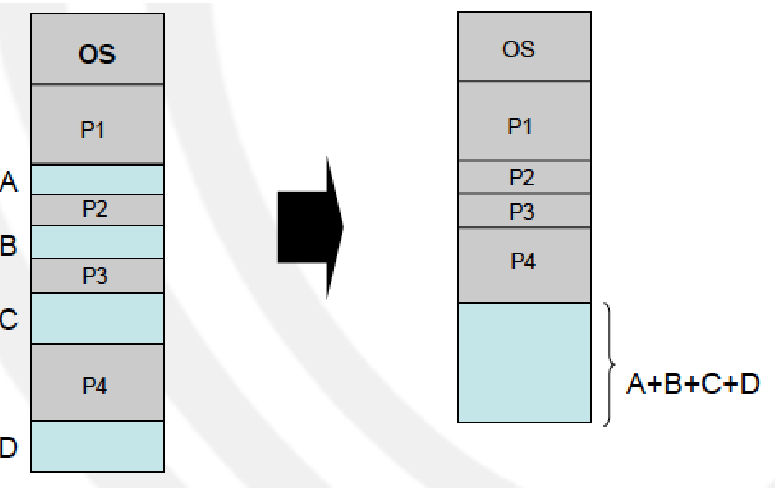
\includegraphics[width=\textwidth]{09/compattazione.png}
                        \caption{Compattazione}
                        \label{fig:compattazione}
                    \end{subfigure}
                    \begin{subfigure}{0.45\textwidth}
                        \centering
                        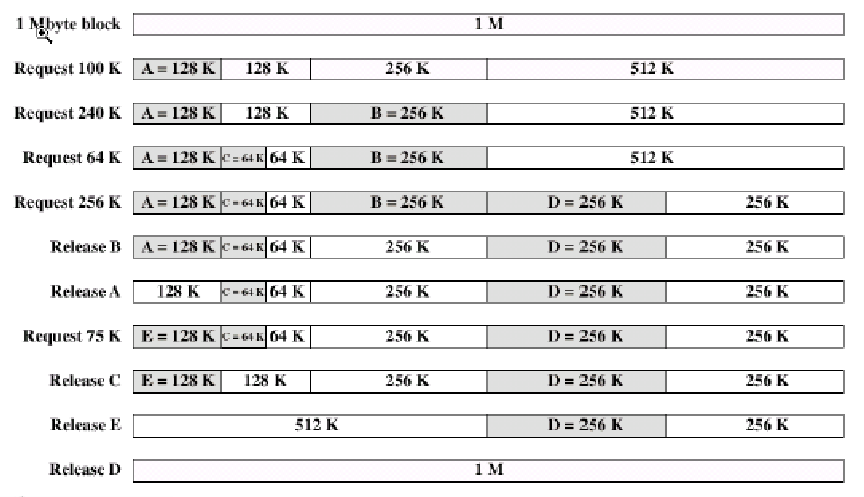
\includegraphics[width=\textwidth]{09/buddySystem.png}
                        \caption{\textit{Buddy-system}}
                        \label{fig:buddySystem}
                    \end{subfigure}
                    \caption{Tecniche di deframmentazione}
                \end{figure}
    \subsection{Paginazione}
        La paginazione è una tecnica per eliminare la frammentazione, sia esterna che interna, si basa sull'idea che lo spazio di indirizzamento di un processo può essere non-contiguo e che la memoria fisica può essere suddivisa in blocchi di dimensioni fisse detti \textit{frame}, mentre la memoria logica viene divisa in blocchi di dimensioni fisse detti \textit{page}.\newline
        Se vogliamo eseguire un programma il quale necessita $n$ pagine allora bisogna trovare $n$ \textit{frame} liberi, indipendentemente che questi siano contigui o meno. Per trovare le pagine libere il \texttt{SO} mantiene una tabella delle pagine, la quale mappa ogni processo alle sue pagine associate agli \textit{frame} fisici.
        \subsubsection{Tabulaizone degli indirizzi}
            Ogni indirizzo logico (generato dalla \texttt{CPU}) viene suddiviso in due parti:
            \begin{itemize}
                \item \textbf{Numero di pagina ($p$)}: il numero della pagina a cui appartiene l'indirizzo logico (se la pagina ha dimensione $2^n$ e la memoria ha dimensione $2^m$ allora il numero di pagina è di $m-n$ bit)
                \item \textbf{Offset ($d$)}: la posizione all'interno della pagina (se la pagina ha dimensione $2^n$ allora l'offset è di $n$ bit)
            \end{itemize}
            L'indirizzo logico viene quindi rappresentato come una coppia di numeri $(p,d)$, dove $p$ è il numero della pagina e $d$ è l'offset. Per ottenere l'indirizzo fisico, il \texttt{SO} deve tradurre il numero di pagina nell'indirizzo base della pagina fisica e sommarlo all'offset. L'indirizzo fisico viene quindi rappresentato come la coppia $(f,d)$ dove $f$ è il numero dell'\textit{frame} e $d$ è l'offset.
        \subsubsection{Implementazioni} 
            Dato che l'efficienza è fondamentale in quanto la traduzione degli indirizzi deve essere eseguita in tempo reale, esistono diverse soluzioni per l'implementazione della traduzione degli indirizzi.
            \paragraph{Implementazione tramite registri}    
                Tutte le \textit{entry} della tabella sono archiviate in un registro, e ogni volta che viene generato un indirizzo logico, il \texttt{SO} deve accedere al registro per ottenere l'indirizzo fisico. Questo tipo di implementazione è molto veloce, ma questo al costo di un numero ridotto di \textit{entry} ed un allungamento dei tempi di \textit{context-switch}.
            \paragraph{Implementazione in memoria} 
                Al posto di memorizzare l'intera tabella delle pagine in un registro, il \texttt{SO} memorizza solo un puntatore alla base della tabella delle pagine in un registro, ed un opzionale registro per la lunghezza della tabella delle pagine. Risulta quindi più veloce il \textit{context-switch} in quanto la variazione riguarda solo il registro \texttt{PTBR} (\textit{Page Table Base Register}) e il registro \texttt{PTLR} (\textit{Page Table Length Register}). Questo però richiede due accessi alla memoria, uno per leggere la tabella delle pagine e uno per leggere l'\textit{frame} fisico. Per ovviare a questo problema si usa una \textit{cache} della tabella delle pagine, chiamata \texttt{TLB} (\textit{Translation Look-aside Buffer}) che memorizza le traduzioni più recenti. La \texttt{TLB} è una memoria veloce che memorizza le traduzioni più recenti e permette di ridurre il numero di accessi alla memoria. Quando viene generato un indirizzo logico, il \texttt{SO} verifica se la traduzione è presente nella \texttt{TLB}, se è presente la traduzione viene eseguita in modo veloce ($<10\%$ rispetto al \textit{lookup} in memoria), altrimenti viene eseguita la traduzione in memoria. \newline
                Il tempo di accesso effettivo medio alla memoria è dato dalla seguente formula:
                \begin{equation*}
                    T_{eff} = T_{TLB} + (1 - p) \cdot T_{mem} + p \cdot (T_{TLB} + T_{mem})
                \end{equation*}
                Dove $T_{TLB}$ è il tempo di accesso alla \texttt{TLB}, $T_{mem}$ è il tempo di accesso alla memoria e $p$ è la probabilità che la traduzione sia presente nella \texttt{TLB}. Se la \texttt{TLB} è molto veloce e la probabilità che la traduzione sia presente è alta, il tempo di accesso effettivo alla memoria sarà molto basso.
        \subsubsection{Protezione}
            La protezione della memoria è implementata associando ad ogni \textit{frame} un bit di protezione, che indica se il \textit{frame} è accessibile o meno. Se un processo tenta di accedere a un \textit{frame} non accessibile, il \texttt{SO} genera un'eccezione e il processo viene terminato. Esistono poi i bit di accesso che determinano se una pagina è modificabile o meno oppure se è eseguibile o meno.
        \subsubsection{Pagine condivise}    
            La paginazione permette di avere più cope virtuali di una pagina in memoria ma una stessa copia fisica, ovvero più processi possono condividere la stessa pagina fisica. Questo permette condividere pagine (\textit{read-only}) tra più processi mantenendo però la protezione della memoria.
        \subsubsection{Spazio di indirizzamento}
            Modernamente gli indirizzi sono o a \texttt{32} o a \texttt{64} bit, e quindi lo spazio di indirizzamento è di $2^{32}$ o $2^{64}$ byte, il quale è molto maggiore dello spazio di indirizzamento fisico. Per questo motivo vengono usati dei meccanismi per gestire il problema della dimensione della tabella delle pagine:
            \begin{itemize}
                \item Paginazione della tabella delle pagine: la tabella delle pagine viene suddivisa in pagine di dimensioni fisse, e ogni pagina della tabella delle pagine viene memorizzata in memoria. Questo permette di ridurre la dimensione della tabella delle pagine e di gestire lo spazio di indirizzamento in modo più efficiente.
                \item Tabella delle pagine invertita: la tabella delle pagine viene memorizzata in memoria e ogni \textit{entry} della tabella delle pagine contiene l'indirizzo fisico della pagina. Questo permette di ridurre la dimensione della tabella delle pagine e di gestire lo spazio di indirizzamento in modo più efficiente.
            \end{itemize}
            La paginazione della tabella delle pagine è più complessa da implementare, ma permette di gestire lo spazio di indirizzamento in modo più efficiente. La tabella delle pagine invertita è più semplice da implementare, ma richiede più memoria e può portare a problemi di frammentazione.\newline
            La paginazione delle tabella delle pagine è una tecnica simile alla paginazione multi-livello, in quanto la tabella delle pagine viene suddivisa in più livelli di pagine. In questo caso la tabella delle pagine è suddivisa in più livelli di pagine, e ogni pagina della tabella delle pagine contiene un puntatore alla pagina successiva.
        \subsubsection{Paginazione con \textit{hashing}}
            La paginazione con \textit{hashing} è una tecnica di gestione della memoria che utilizza una funzione di \textit{hashing} per restituire l'indirizzo fisico di una pagina. Riducendo il costo di ricerca delle pagine da $O(n)$ a $O(1)$, la paginazione con \textit{hashing} è più veloce rispetto alla paginazione tradizionale. 
\section{Segmentazione}
    La segmentazione è una tecnica di gestione della memoria che permette di suddividere la memoria in segmenti di dimensioni variabili. Ogni segmento rappresenta un'unità logica del programma, come ad esempio una funzione o una variabile globale. La segmentazione permette di gestire la memoria in modo più flessibile rispetto alla paginazione, in quanto i segmenti possono avere dimensioni diverse e possono essere allocati in modo non contiguo.\newline
    La segmentazione è simile alla paginazione, ma invece di suddividere la memoria in pagine di dimensioni fisse, la segmentazione suddivide la memoria in segmenti di dimensioni variabili. L'indirizzo logico viene quindi rappresentato come una coppia di numeri $(s,d)$, dove $s$ è il numero del segmento e $d$ è l'offset. Per ottenere l'indirizzo fisico, il \texttt{SO} deve tradurre il numero del segmento nell'indirizzo base del segmento fisico e sommarlo all'offset. La tabella dei segmenti è simile alla tabella delle pagine, ma invece di memorizzare gli indirizzi fisici delle pagine, la tabella dei segmenti memorizza gli indirizzi fisici dei segmenti (base e limite). Anche per questa tabella esiste una \texttt{STBR} (\textit{Segment Table Base Register}) e una \texttt{STLR} (\textit{Segment Table Length Register}).\newline
    Prima di tradurre un indirizzo logico in un indirizzo fisico, il \texttt{SO} deve verificare se il numero del segmento è valido e se l'offset è compreso tra $0$ e la dimensione del segmento. Se il numero del segmento è valido e l'offset è compreso tra $0$ e la dimensione del segmento, il \texttt{SO} traduce l'indirizzo logico in un indirizzo fisico sommando l'indirizzo base del segmento all'offset. Se il numero del segmento non è valido o l'offset non è compreso tra $0$ e la dimensione del segmento, il \texttt{SO} genera un'eccezione e il processo viene terminato.
    \paragraph{Protezione}
        Anche la segmentazione prevede l'uso di bit di protezione, che indicano se il segmento è accessibile o meno. Se un processo tenta di accedere a un segmento non accessibile, il \texttt{SO} genera un'eccezione e il processo viene terminato. Inoltre i segmenti possono essere protetti in modo da impedire la scrittura o la lettura da parte di altri processi.
    \paragraph{Segmenti condivisi}
        La segmentazione permette di avere più copie virtuali di un segmento in memoria ma una sola copia fisica, ovvero più processi possono condividere lo stesso segmento fisico. Questo permette di condividere segmenti (\textit{read-only}) tra più processi mantenendo però la protezione della memoria.
    \paragraph{Segmentazione e frammentazione}
        Il sistema operativo deve allocare spazio in memoria per tutti i segmenti di un processo, e se un segmento richiede più memoria di quella disponibile, il processo non può essere caricato in memoria finché non viene liberato un segmento di dimensioni sufficienti. Questo porta a problemi di frammentazione esterna, in quanto i segmenti possono essere allocati in modo non contiguo e possono portare a problemi di frammentazione interna.
    \subsubsection{Paginazione v/s segmentazione}
        La paginazione e la segmentazione sono due tecniche di gestione della memoria che hanno vantaggi e svantaggi diversi. La paginazione permette una non esistenza di frammentazione (poca interna) ed l'allocazione dei frame non richiede uno specifico algoritmo. D'altro canto la segmentazione permette una maggiore consistenza tra vista fisica della memoria e vista logica della memoria, oltre alla associazione di protezione e condivisione a livello di segmento e non a livello di pagina. Tra gli svantaggi della segmentazione c'è la frammentazione esterna e la necessità di un algoritmo di allocazione per i segmenti dinamica, mentre tra gli svantaggi della paginazione c'è la separazione tra vista fisica e logica della memoria, la necessità di una tabella delle pagine e la frammentazione interna.
\section{Segmentazione con paginazione}
    Una soluzione per eliminare i problemi di frammentazione esterna e interna è la segmentazione con paginazione combinando le due tecniche. In questo caso la memoria viene suddivisa in segmenti di dimensioni variabili e ogni segmento viene suddiviso in pagine di dimensioni fisse. Ogni segmento rappresenta un'unità logica del programma, come ad esempio una funzione o una variabile globale, mentre le pagine rappresentano l'unità fisica di allocazione della memoria.
    \paragraph{\texttt{MULTICS}}
        Il sistema operativo \texttt{MULTICS} è un esempio di sistema operativo che utilizza la segmentazione con paginazione. In questo caso la memoria viene suddivisa in segmenti di dimensioni variabili e ogni segmento viene suddiviso in pagine di dimensioni fisse. Ogni segmento rappresenta un'unità logica del programma, come ad esempio una funzione o una variabile globale, mentre le pagine rappresentano l'unità fisica di allocazione della memoria. La tabella dei segmenti è simile alla tabella delle pagine, ma invece di memorizzare gli indirizzi fisici delle pagine, la tabella dei segmenti memorizza gli indirizzi fisici dei segmenti (base e limite). Anche per questa tabella esiste una \texttt{STBR} (\textit{Segment Table Base Register}) e una \texttt{STLR} (\textit{Segment Table Length Register}).\newline
        La traduzione degli indirizzi logici in indirizzi fisici avviene in due passaggi:
        \begin{itemize}
            \item Il numero del segmento viene tradotto nell'indirizzo base del segmento fisico e l'offset viene sommato all'indirizzo base del segmento per ottenere l'indirizzo fisico della pagina.
            \item Il numero della pagina viene tradotto nell'indirizzo base della pagina fisica e l'offset viene sommato all'indirizzo base della pagina per ottenere l'indirizzo fisico.
        \end{itemize}
        In questo modo la segmentazione con paginazione permette di gestire la memoria in modo più flessibile rispetto alla paginazione e alla segmentazione, eliminando i problemi di frammentazione esterna e interna.
    \paragraph{\texttt{ARMv7-A}}
        Nella tecnologia \texttt{ARMv7-A} la segmentazione con paginazione è implementata divisa in quattro dimensioni:
        \begin{itemize}
            \item Super-Sezioni: $16MB$ di memoria fisica ($24bit$ di offset)
            \item Sezioni: $1MB$ di memoria fisica ($20bit$ di offset)
            \item Pagine grandi: $64KB$ di memoria fisica ($16bit$ di offset)
            \item Pagine piccole: $4KB$ di memoria fisica ($12bit$ di offset)
        \end{itemize}
        Ogni \textit{entry} della tabella delle pagine può contenere o l'indirizzo direttamente di una sezione, oppure un puntatore al secondo livello della tabella delle pagine. Inoltre \texttt{ARM} ha due livelli di \texttt{TLB}:
        \begin{itemize}
            \item \texttt{L1 TLB}: piccola e veloce, memorizza le traduzioni più recenti. (32 \textit{entry})
            \item \texttt{L2 TLB}: più grande e lenta, memorizza le traduzioni meno recenti. (8+64 \textit{entry})
        \end{itemize}